\documentclass[12pt,a4paper]{article}
\usepackage[utf8]{inputenc}
\usepackage[spanish]{babel}
\usepackage{amsmath}
\usepackage{amsfonts}
\usepackage{amssymb}
\usepackage{graphicx}
\usepackage[left=2cm,right=2cm,top=2cm,bottom=2cm]{geometry}

\usepackage{enumitem}
\usepackage{algorithm}
\usepackage{algorithmic}
\usepackage[hidelinks]{hyperref}

\usepackage{tikz}

\usepackage{subcaption}
\usepackage{pgfplots}

% Para la tabla
\usepackage[normalem]{ulem}
\useunder{\uline}{\ul}{}


\author{Ignacio Aguilera Martos}
\title{Práctica 2 \\ Técnicas de los Sistemas Inteligentes}
\date{\today}

\setlength{\parindent}{0cm}
\setlength{\parskip}{10px}


\begin{document}
	\maketitle

	\tableofcontents

	\newpage

\section{Ejercicio 1}

El primero de los apartados nos pide definir los objetos, personajes y demás tipos utilizados en el dominio. Los tipos que yo he representado son zona, orientación, agente, princesa, principe, bruja, profesor, leonardo, oscar, manzana, rosa, algoritmo, oro, personaje, objeto y posicionable.

El diagrama de tipos que he empleado es un árbol de la forma:

\begin{figure}[H]
	\centering
	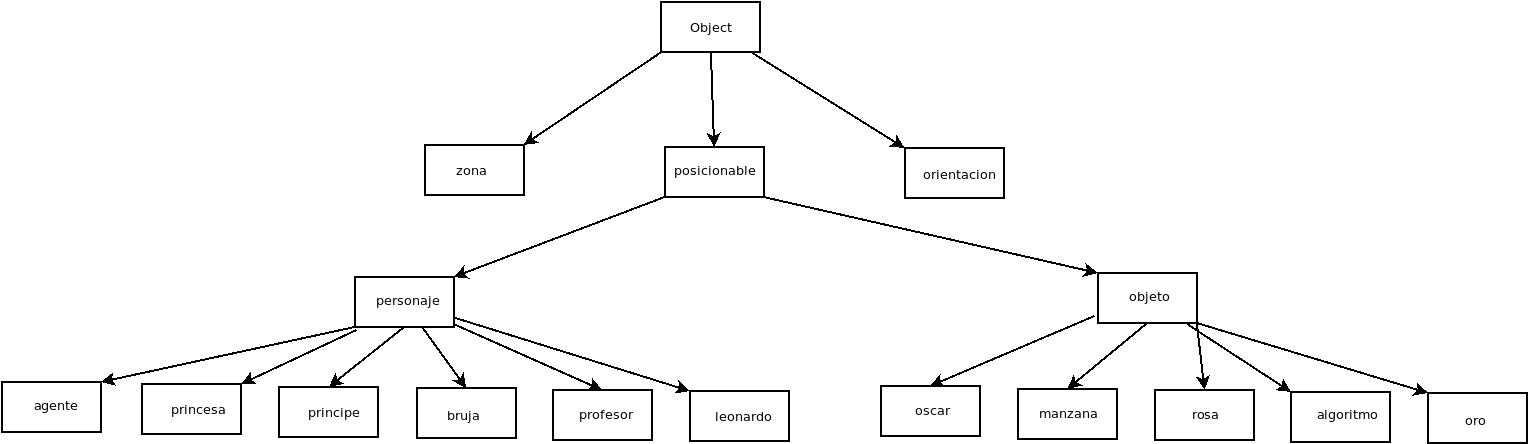
\includegraphics[scale=0.32]{./Imagenes/diag-ej1.png}
	\caption{Diagrama de tipos}
\end{figure}

En cuanto a los predicados que he tomado para resolver el ejercicio son:

\begin{itemize}
	\item (en ?x - posicionable ?y - zona): este predicado lo que nos indica es que el objeto o personaje ?x está en la zona ?y.
	\item (orientado ?a - personaje ?ori - orientacion): este predicado nos dice que el personaje (incluido el propio agente) ?a está orientado según la orientación ?ori.
	\item (conectado ?z1 ?z2 - zona ?ori - orientacion): este predicado nos dice que las zonas ?z1 y ?z2 están conectadas por la orientación ?ori, esto es si z2 está a la derecha de z1 entonces están conectadas por el este, si z2 está debajo de z1 entonces z1 está conectada a z2 por el sur y así para el resto de orientaciones.
	\item (manovacia ?a - agente): este predicado nos dice si el agente ?a tiene o no la mano vacía para llevar un objeto.
	\item (enlamano ?a - agente ?obj - objeto): este predicado nos dice que el agente ?a tiene un objeto ?obj en la mano.
	\item (tieneobjeto ?per - personaje): este predicado nos indica que el personaje ?per tiene un objeto.
\end{itemize}

Cabe decir que además de los predicados y tipos he definido 4 constantes para las orientaciones que son este, oeste, norte y sur.

Para las acciones las he definido de la siguiente forma:

\begin{itemize}
	\item girar-izquierda: es la acción que nos permite rotar hacia la izquierda, requiere como único parámetro un agente y el efecto es, comprobando la orientación actual del agente cambiar dicha orientación de forma adecuada al giro a la izquierda.
	\item girar-derecha: es la misma acción que girar a la izquierda pero cambiando el sentido de la rotación.
	\item ir: recibe como parámetros un agente, dos zonas y una orientación. Como precondiciones establecemos que el agente esté en la primera de las posiciones, que el agente esté orientado según la orientación dada y que las zonas estén conectadas en esa dirección. El efecto de esta acción es que el agente pasa a estar en la segunda zona y deja de estar en la primera.
	\item coger: esta acción recibe como parámetros un agente, una zona y un objeto. Se pide como precondición que el agente esté en la zona, el objeto también y que el agente tenga la mano vacía. Como efecto se produce que el agente deja de tener la mano vacía, el objeto deja de estar en la zona y pasa a estar en la mano del agente.
	\item dejar: recibe como parámetros un agente, una zona y un objeto. Como precondiciones se pide que el agente esté en la posición y tenga el objeto en la mano. El efecto que se produce es que el objeto pasa a estar en la zona y desaparece de la mano del agente y éste pasa a tener la mano vacía.
	\item entregar: recibe como parámetros un agente, una zona, un objeto y un personaje. Como precondiciones se pide que el agente esté en la zona, el personaje también y que el agente tenga el objeto en la mano. El efecto producido es que el agente deja de tener el objeto en la mano, pasa a tener la mano vacía y el objeto pasa a tenerlo el personaje.
\end{itemize}

Lo siguiente que se nos pide es que planteemos de forma manual un problema con 25 zonas, 5 personajes mas el agente y 5 objetos. El objetivo será que cada uno de los 5 personajes tenga un objeto.

La disposición del mapa que he dado es la siguiente:

\tikzset{every picture/.style={line width=0.75pt}} %set default line width to 0.75pt

\begin{tikzpicture}[x=0.75pt,y=0.75pt,yscale=-0.9,xscale=0.9][H]
%uncomment if require: \path (0,722); %set diagram left start at 0, and has height of 722

%Shape: Grid [id:dp8007827105902172]
\draw  [draw opacity=0][fill={rgb, 255:red, 255; green, 255; blue, 255 }  ,fill opacity=1 ] (35,24) -- (795,24) -- (795,499) -- (35,499) -- cycle ; \draw  [color={rgb, 255:red, 75; green, 75; blue, 75 }  ,draw opacity=1 ] (130,24) -- (130,499)(225,24) -- (225,499)(320,24) -- (320,499)(415,24) -- (415,499)(510,24) -- (510,499)(605,24) -- (605,499)(700,24) -- (700,499) ; \draw  [color={rgb, 255:red, 75; green, 75; blue, 75 }  ,draw opacity=1 ] (35,119) -- (795,119)(35,214) -- (795,214)(35,309) -- (795,309)(35,404) -- (795,404) ; \draw  [color={rgb, 255:red, 75; green, 75; blue, 75 }  ,draw opacity=1 ] (35,24) -- (795,24) -- (795,499) -- (35,499) -- cycle ;

% Text Node
\draw (68,64) node  [align=left] {Agente};
% Text Node
\draw (265,63) node  [align=left] {Princesa};
% Text Node
\draw (53,38) node  [align=left] {z1};
% Text Node
\draw (148,42) node  [align=left] {z2};
% Text Node
\draw (245,35) node  [align=left] {z3};
% Text Node
\draw (336,38) node  [align=left] {z4};
% Text Node
\draw (433,42) node  [align=left] {z5};
% Text Node
\draw (56,133) node  [align=left] {z6};
% Text Node
\draw (149,133) node  [align=left] {z7};
% Text Node
\draw (244,133) node  [align=left] {z8};
% Text Node
\draw (339,133) node  [align=left] {z9};
% Text Node
\draw (436,136) node  [align=left] {z10};
% Text Node
\draw (56,232) node  [align=left] {z11};
% Text Node
\draw (152,230) node  [align=left] {z12};
% Text Node
\draw (244,232) node  [align=left] {z13};
% Text Node
\draw (343,232) node  [align=left] {z14};
% Text Node
\draw (439,230) node  [align=left] {z15};
% Text Node
\draw (56,325) node  [align=left] {z16};
% Text Node
\draw (152,326) node  [align=left] {z17};
% Text Node
\draw (247,327) node  [align=left] {z18};
% Text Node
\draw (341,323) node  [align=left] {z19};
% Text Node
\draw (438,323) node  [align=left] {z20};
% Text Node
\draw (535,325) node  [align=left] {z21};
% Text Node
\draw (625,324) node  [align=left] {z22};
% Text Node
\draw (720,322) node  [align=left] {z23};
% Text Node
\draw (717,419) node  [align=left] {z24};
% Text Node
\draw (720,231) node  [align=left] {z25};
% Text Node
\draw (258,159) node  [align=left] {Oscar};
% Text Node
\draw (453,68) node  [align=left] {Principe};
% Text Node
\draw (63,154) node  [align=left] {Oro};
% Text Node
\draw (458,159) node  [align=left] {Leonardo};
% Text Node
\draw (61,257) node  [align=left] {Bruja};
% Text Node
\draw (362,259) node  [align=left] {Manzana};
% Text Node
\draw (267,348) node  [align=left] {Profesor};
% Text Node
\draw (542,352) node  [align=left] {Rosa};
% Text Node
\draw (745,346) node  [align=left] {Algoritmo};
\end{tikzpicture}

Partimos además de que el agente está orientado hacia el norte, tiene la mano vacía y el objetivo es que todos los personajes tengan un objeto.

Por último se nos pide un parser que he implementado en Python3 que dada una entrada de la forma:

numero de zonas:7

Dominio:Ejercicio2

Problema:Problema2

V -$>$ z1[bruja1-bruja] z3[] z6[]

H -$>$ z2[player1-agente] z3[] z4[]

H -$>$ z5[oscar1-oscar,manzana1-manzana] z6[] z7[princesa1-princesa]

Cabe decir que tenemos que poner los nombres de los tipos en minúscula para que casen con los que yo he definido.

Además, aunque el enunciado dice que los objetos de cada zona (entre corchetes) deben estar separados por espacios, he tomado la decisión de diseño de que los elementos estén separados por comas, pues de  esta forma los separadores son únicos para cada caso lo que hace que su división sea más sencilla.

El resto es simplemente un programa en Python comentado que convierte este fichero en un fichero de problema PDDL completo usando el dominio descrito anteriormente.

\section{Ejercicio 2}

Para ajustar el dominio al nuevo problema tenemos que definir dos funciones:

\begin{itemize}
	\item (coste ?z1 ?z2): nos indica cuál es el coste de pasar de la zona ?z1 a la zona ?z2.
	\item (costeTotal): es la suma del coste del camino que estamos recorriendo, es decir, cada vez que entremos a la acción ir sumaremos a esta función el coste del arco (coste ?z1 ?z2) tomado.
\end{itemize}

Para terminar de adecuar esto tenemos que modificar la función ``ir'' para que en los efectos se incremente (costeTotal) de la forma (increase (costeTotal) (coste ?z1 ?z2)) donde ``ir'' parte de que el agente está en la zona ?z1 y quiere desplazarse a la zona ?z2.

Para la extensión del problema podemos tomar todo lo hecho y únicamente añadir en el bloque ``init'' la declaración de los pesos de las conexiones e inicializar (costeTotal) a 0.

En el problema anterior de 25 zonas vamos a añadir los siguientes pesos:

\tikzset{every picture/.style={line width=0.75pt}} %set default line width to 0.75pt

\begin{tikzpicture}[x=0.75pt,y=0.75pt,yscale=-0.9,xscale=0.9][H]
%uncomment if require: \path (0,722); %set diagram left start at 0, and has height of 722

%Shape: Grid [id:dp8007827105902172]
\draw  [draw opacity=0][fill={rgb, 255:red, 255; green, 255; blue, 255 }  ,fill opacity=1 ] (35,24) -- (795,24) -- (795,499) -- (35,499) -- cycle ; \draw  [color={rgb, 255:red, 75; green, 75; blue, 75 }  ,draw opacity=1 ] (130,24) -- (130,499)(225,24) -- (225,499)(320,24) -- (320,499)(415,24) -- (415,499)(510,24) -- (510,499)(605,24) -- (605,499)(700,24) -- (700,499) ; \draw  [color={rgb, 255:red, 75; green, 75; blue, 75 }  ,draw opacity=1 ] (35,119) -- (795,119)(35,214) -- (795,214)(35,309) -- (795,309)(35,404) -- (795,404) ; \draw  [color={rgb, 255:red, 75; green, 75; blue, 75 }  ,draw opacity=1 ] (35,24) -- (795,24) -- (795,499) -- (35,499) -- cycle ;

% Text Node
\draw (68,64) node  [align=left] {Agente};
% Text Node
\draw (265,63) node  [align=left] {Princesa};
% Text Node
\draw (53,38) node  [align=left] {z1};
% Text Node
\draw (148,42) node  [align=left] {z2};
% Text Node
\draw (245,35) node  [align=left] {z3};
% Text Node
\draw (336,38) node  [align=left] {z4};
% Text Node
\draw (433,42) node  [align=left] {z5};
% Text Node
\draw (56,133) node  [align=left] {z6};
% Text Node
\draw (149,133) node  [align=left] {z7};
% Text Node
\draw (244,133) node  [align=left] {z8};
% Text Node
\draw (339,133) node  [align=left] {z9};
% Text Node
\draw (436,136) node  [align=left] {z10};
% Text Node
\draw (56,232) node  [align=left] {z11};
% Text Node
\draw (152,230) node  [align=left] {z12};
% Text Node
\draw (244,232) node  [align=left] {z13};
% Text Node
\draw (343,232) node  [align=left] {z14};
% Text Node
\draw (439,230) node  [align=left] {z15};
% Text Node
\draw (56,325) node  [align=left] {z16};
% Text Node
\draw (152,326) node  [align=left] {z17};
% Text Node
\draw (247,327) node  [align=left] {z18};
% Text Node
\draw (341,323) node  [align=left] {z19};
% Text Node
\draw (438,323) node  [align=left] {z20};
% Text Node
\draw (535,325) node  [align=left] {z21};
% Text Node
\draw (625,324) node  [align=left] {z22};
% Text Node
\draw (720,322) node  [align=left] {z23};
% Text Node
\draw (717,419) node  [align=left] {z24};
% Text Node
\draw (720,231) node  [align=left] {z25};
% Text Node
\draw (131,72) node  [align=left] {5};
% Text Node
\draw (227,78) node  [align=left] {4};
% Text Node
\draw (321,77) node  [align=left] {3};
% Text Node
\draw (415,81) node  [align=left] {8};
% Text Node
\draw (89,119) node  [align=left] {2};
% Text Node
\draw (174,117) node  [align=left] {5};
% Text Node
\draw (274,118) node  [align=left] {6};
% Text Node
\draw (370,118) node  [align=left] {5};
% Text Node
\draw (470,118) node  [align=left] {2};
% Text Node
\draw (130,160) node  [align=left] {3};
% Text Node
\draw (225,165) node  [align=left] {6};
% Text Node
\draw (321,165) node  [align=left] {5};
% Text Node
\draw (415,167) node  [align=left] {1};
% Text Node
\draw (84,215) node  [align=left] {1};
% Text Node
\draw (174,213) node  [align=left] {1};
% Text Node
\draw (273,215) node  [align=left] {1};
% Text Node
\draw (371,213) node  [align=left] {1};
% Text Node
\draw (467,216) node  [align=left] {1};
% Text Node
\draw (130,260) node  [align=left] {7};
% Text Node
\draw (227,264) node  [align=left] {2};
% Text Node
\draw (321,261) node  [align=left] {6};
% Text Node
\draw (414,264) node  [align=left] {2};
% Text Node
\draw (82,308) node  [align=left] {4};
% Text Node
\draw (179,309) node  [align=left] {3};
% Text Node
\draw (277,308) node  [align=left] {2};
% Text Node
\draw (370,307) node  [align=left] {6};
% Text Node
\draw (469,306) node  [align=left] {8};
% Text Node
\draw (130,355) node  [align=left] {8};
% Text Node
\draw (227,352) node  [align=left] {9};
% Text Node
\draw (321,356) node  [align=left] {2};
% Text Node
\draw (414,357) node  [align=left] {5};
% Text Node
\draw (512,359) node  [align=left] {2};
% Text Node
\draw (606,357) node  [align=left] {1};
% Text Node
\draw (701,357) node  [align=left] {4};
% Text Node
\draw (755,309) node  [align=left] {8};
% Text Node
\draw (751,403) node  [align=left] {6};
% Text Node
\draw (258,159) node  [align=left] {Oscar};
% Text Node
\draw (453,68) node  [align=left] {Principe};
% Text Node
\draw (63,154) node  [align=left] {Oro};
% Text Node
\draw (458,159) node  [align=left] {Leonardo};
% Text Node
\draw (61,257) node  [align=left] {Bruja};
% Text Node
\draw (362,259) node  [align=left] {Manzana};
% Text Node
\draw (267,348) node  [align=left] {Profesor};
% Text Node
\draw (542,352) node  [align=left] {Rosa};
% Text Node
\draw (745,346) node  [align=left] {Algoritmo};
\end{tikzpicture}

\section{Ejercicio 3}

En primer lugar, para representar los tipos de terrenos he declarado un nuevo tipo llamado ``superficie'' del que he declarado las constantes: bosque, agua, precipicio, arena y piedra. Además he declarado los tipos bikini y zapatilla que son subtipos de objeto con lo que se considera que los bikinis y zapatillas también son objetos.

Para poder representar esta nueva información he añadido el predicado (es ?sup ?z) que nos indica que la zona ?z es del tipo de superficie ?sup y los predicados (esbikini ?obj) y (eszapatilla ?obj) que nos indican si los objetos son zapatillas o bikinis.

Para representar el conocimiento de la mochila ahora tenemos dos predicados nuevos que son (mochilavacia ?age) que nos dice que el agente ?age tiene la mochila vacía y (enlamochila ?age ?obj) que nos dice que el agente ?age tiene el objeto ?obj en la mochila.

En cuanto a las acciones que han sido modificadas son dos ``ir'' y las nuevas acciones de ``meter-mochila'' y ``sacar-mochila''.

La acción de ir ahora tiene nuevas precondiciones. Sumadas a las anteriores se pide ahora que la zona a la que se va a ir no sea precipicio, que no sea agua o que en caso de serlo tengamos un bikini en la mochila o en la mano y que o no sea bosque o que si lo es tengamos unas zapatillas en la mochila o en la mano. De esta forma no nos moveremos a los precipicios y sólo pasaremos por el agua con un bikini y por el bosque con unas zapatillas.

La acción ``meter-mochila'' requiere que tengamos un objeto en la mano y la mochila vacía. Como efecto se cumple que tenemos la mano vacía, el objeto en la mochila y ya no tenemos la mochila vacía ni el objeto en la mano.

La acción ``sacar-mochila'' requiere que tengamos un objeto en la mochila y la mano vacía. Como efecto se cumple que tenemos la mochila vacía, el objeto en la mano y ya no tenemos la mano vacía ni el objeto en la mochila.

El problema para ser extendido requiere que definamos las superficies de cada zona y añadamos un bikini y unas zapatillas al menos, con lo que el mapa queda:

\tikzset{every picture/.style={line width=0.75pt}} %set default line width to 0.75pt

\begin{tikzpicture}[x=0.75pt,y=0.75pt,yscale=-0.9,xscale=0.9][H]
%uncomment if require: \path (0,722); %set diagram left start at 0, and has height of 722

%Shape: Grid [id:dp8007827105902172]
\draw  [draw opacity=0][fill={rgb, 255:red, 255; green, 255; blue, 255 }  ,fill opacity=1 ] (35,23) -- (795,23) -- (795,498) -- (35,498) -- cycle ; \draw  [color={rgb, 255:red, 75; green, 75; blue, 75 }  ,draw opacity=1 ] (130,23) -- (130,498)(225,23) -- (225,498)(320,23) -- (320,498)(415,23) -- (415,498)(510,23) -- (510,498)(605,23) -- (605,498)(700,23) -- (700,498) ; \draw  [color={rgb, 255:red, 75; green, 75; blue, 75 }  ,draw opacity=1 ] (35,118) -- (795,118)(35,213) -- (795,213)(35,308) -- (795,308)(35,403) -- (795,403) ; \draw  [color={rgb, 255:red, 75; green, 75; blue, 75 }  ,draw opacity=1 ] (35,23) -- (795,23) -- (795,498) -- (35,498) -- cycle ;

% Text Node
\draw (68,64) node  [align=left] {\textcolor[rgb]{0.82,0.01,0.11}{Agente}};
% Text Node
\draw (265,63) node  [align=left] {\textcolor[rgb]{0.82,0.01,0.11}{Princesa}};
% Text Node
\draw (53,38) node  [align=left] {z1};
% Text Node
\draw (148,42) node  [align=left] {z2};
% Text Node
\draw (245,35) node  [align=left] {z3};
% Text Node
\draw (336,38) node  [align=left] {z4};
% Text Node
\draw (433,42) node  [align=left] {z5};
% Text Node
\draw (56,133) node  [align=left] {z6};
% Text Node
\draw (149,133) node  [align=left] {z7};
% Text Node
\draw (244,133) node  [align=left] {z8};
% Text Node
\draw (339,133) node  [align=left] {z9};
% Text Node
\draw (436,136) node  [align=left] {z10};
% Text Node
\draw (56,232) node  [align=left] {z11};
% Text Node
\draw (152,230) node  [align=left] {z12};
% Text Node
\draw (244,232) node  [align=left] {z13};
% Text Node
\draw (343,232) node  [align=left] {z14};
% Text Node
\draw (439,230) node  [align=left] {z15};
% Text Node
\draw (56,325) node  [align=left] {z16};
% Text Node
\draw (152,326) node  [align=left] {z17};
% Text Node
\draw (247,327) node  [align=left] {z18};
% Text Node
\draw (341,323) node  [align=left] {z19};
% Text Node
\draw (438,323) node  [align=left] {z20};
% Text Node
\draw (535,325) node  [align=left] {z21};
% Text Node
\draw (625,324) node  [align=left] {z22};
% Text Node
\draw (720,322) node  [align=left] {z23};
% Text Node
\draw (717,419) node  [align=left] {z24};
% Text Node
\draw (720,231) node  [align=left] {z25};
% Text Node
\draw (131,72) node  [align=left] {5};
% Text Node
\draw (227,78) node  [align=left] {4};
% Text Node
\draw (321,77) node  [align=left] {3};
% Text Node
\draw (415,81) node  [align=left] {8};
% Text Node
\draw (89,119) node  [align=left] {2};
% Text Node
\draw (174,117) node  [align=left] {5};
% Text Node
\draw (274,118) node  [align=left] {6};
% Text Node
\draw (370,118) node  [align=left] {5};
% Text Node
\draw (470,118) node  [align=left] {2};
% Text Node
\draw (130,160) node  [align=left] {3};
% Text Node
\draw (225,165) node  [align=left] {6};
% Text Node
\draw (321,165) node  [align=left] {5};
% Text Node
\draw (415,167) node  [align=left] {1};
% Text Node
\draw (84,215) node  [align=left] {1};
% Text Node
\draw (174,213) node  [align=left] {1};
% Text Node
\draw (273,215) node  [align=left] {1};
% Text Node
\draw (371,213) node  [align=left] {1};
% Text Node
\draw (467,216) node  [align=left] {1};
% Text Node
\draw (130,260) node  [align=left] {7};
% Text Node
\draw (227,264) node  [align=left] {2};
% Text Node
\draw (321,261) node  [align=left] {6};
% Text Node
\draw (414,264) node  [align=left] {2};
% Text Node
\draw (82,308) node  [align=left] {4};
% Text Node
\draw (179,309) node  [align=left] {3};
% Text Node
\draw (277,308) node  [align=left] {2};
% Text Node
\draw (370,307) node  [align=left] {6};
% Text Node
\draw (469,306) node  [align=left] {8};
% Text Node
\draw (130,355) node  [align=left] {8};
% Text Node
\draw (227,352) node  [align=left] {9};
% Text Node
\draw (321,356) node  [align=left] {2};
% Text Node
\draw (414,357) node  [align=left] {5};
% Text Node
\draw (512,359) node  [align=left] {2};
% Text Node
\draw (606,357) node  [align=left] {1};
% Text Node
\draw (701,357) node  [align=left] {4};
% Text Node
\draw (755,309) node  [align=left] {8};
% Text Node
\draw (751,403) node  [align=left] {6};
% Text Node
\draw (258,159) node  [align=left] {\textcolor[rgb]{0.82,0.01,0.11}{Oscar}};
% Text Node
\draw (453,68) node  [align=left] {\textcolor[rgb]{0.82,0.01,0.11}{Principe}};
% Text Node
\draw (63,154) node  [align=left] {\textcolor[rgb]{0.82,0.01,0.11}{Oro}};
% Text Node
\draw (458,159) node  [align=left] {\textcolor[rgb]{0.82,0.01,0.11}{Leonardo}};
% Text Node
\draw (61,257) node  [align=left] {\textcolor[rgb]{0.82,0.01,0.11}{Bruja}};
% Text Node
\draw (361,259) node  [align=left] {\textcolor[rgb]{0.82,0.01,0.11}{Manzana}};
% Text Node
\draw (267,348) node  [align=left] {\textcolor[rgb]{0.82,0.01,0.11}{Profesor}};
% Text Node
\draw (542,352) node  [align=left] {\textcolor[rgb]{0.82,0.01,0.11}{Rosa}};
% Text Node
\draw (745,346) node  [align=left] {\textcolor[rgb]{0.82,0.01,0.11}{Algoritmo}};
% Text Node
\draw (63,347) node  [align=left] {\textcolor[rgb]{0.82,0.01,0.11}{Bikini}};
% Text Node
\draw (454,254) node  [align=left] {\textcolor[rgb]{0.82,0.01,0.11}{Zapatilla}};
% Text Node
\draw (67,89) node  [align=left] {\textcolor[rgb]{0.29,0.56,0.89}{Piedra}};
% Text Node
\draw (160,87) node  [align=left] {\textcolor[rgb]{0.29,0.56,0.89}{Piedra}};
% Text Node
\draw (256,97) node  [align=left] {\textcolor[rgb]{0.29,0.56,0.89}{Agua}};
% Text Node
\draw (350,95) node  [align=left] {\textcolor[rgb]{0.29,0.56,0.89}{Piedra}};
% Text Node
\draw (450,98) node  [align=left] {\textcolor[rgb]{0.29,0.56,0.89}{Bosque}};
% Text Node
\draw (67,182) node  [align=left] {\textcolor[rgb]{0.29,0.56,0.89}{Arena}};
% Text Node
\draw (160,188) node  [align=left] {\textcolor[rgb]{0.29,0.56,0.89}{Arena}};
% Text Node
\draw (252,189) node  [align=left] {\textcolor[rgb]{0.29,0.56,0.89}{Arena}};
% Text Node
\draw (352,189) node  [align=left] {\textcolor[rgb]{0.29,0.56,0.89}{Arena}};
% Text Node
\draw (447,191) node  [align=left] {\textcolor[rgb]{0.29,0.56,0.89}{Arena}};
% Text Node
\draw (61,284) node  [align=left] {\textcolor[rgb]{0.29,0.56,0.89}{Agua}};
% Text Node
\draw (157,281) node  [align=left] {\textcolor[rgb]{0.29,0.56,0.89}{Piedra}};
% Text Node
\draw (257,284) node  [align=left] {\textcolor[rgb]{0.29,0.56,0.89}{Piedra}};
% Text Node
\draw (351,287) node  [align=left] {\textcolor[rgb]{0.29,0.56,0.89}{Piedra}};
% Text Node
\draw (441,284) node  [align=left] {\textcolor[rgb]{0.29,0.56,0.89}{Agua}};
% Text Node
\draw (61,377) node  [align=left] {\textcolor[rgb]{0.29,0.56,0.89}{Arena}};
% Text Node
\draw (162,376) node  [align=left] {\textcolor[rgb]{0.29,0.56,0.89}{Arena}};
% Text Node
\draw (253,378) node  [align=left] {\textcolor[rgb]{0.29,0.56,0.89}{Arena}};
% Text Node
\draw (447,380) node  [align=left] {\textcolor[rgb]{0.29,0.56,0.89}{Arena}};
% Text Node
\draw (636,376) node  [align=left] {\textcolor[rgb]{0.29,0.56,0.89}{Arena}};
% Text Node
\draw (361,378) node  [align=left] {\textcolor[rgb]{0.29,0.56,0.89}{Precipicio}};
% Text Node
\draw (547,383) node  [align=left] {\textcolor[rgb]{0.29,0.56,0.89}{Bosque}};
% Text Node
\draw (728,283) node  [align=left] {\textcolor[rgb]{0.29,0.56,0.89}{Piedra}};
% Text Node
\draw (733,385) node  [align=left] {\textcolor[rgb]{0.29,0.56,0.89}{Piedra}};
% Text Node
\draw (729,474) node  [align=left] {\textcolor[rgb]{0.29,0.56,0.89}{Piedra}};
\end{tikzpicture}

En este caso para el parser he modificado un poco la sintaxis para adecuarla de la siguiente forma:

numero de zonas:7

Dominio:Ejercicio3

Problema:Problema3

V -$>$ z1[bruja1-bruja](bosque)=10=z3[bikini1-bikini](arena)=5=z6[zapatilla1-zapatilla](piedra)

H -$>$ z2[player1-agente](piedra)=10=z3[](arena)=5=z4[](piedra)

H -$>$ z5[oscar1-oscar,manzana1-manzana](bosque)=10=z6[](piedra)=5=z7[princesa1-princesa](piedra)

Con lo que para el tipo de terreno lo situamos después de los personajes y objetos entre paréntesis. El cambio de corchetes a paréntesis es por simplicidad, puesto que son separadores distintos a los usados hasta el momento y por tanto podemos reutilizar de mejor manera el código previo.

\section{Ejercicio 4}

Para poder mantener un registro de los puntos del agente debemos declarar dos nuevas funciones. La primera de ellas es (puntosTotales) que mantendrá el conteo del número de puntos que lleva el agente por el momento y la función (puntos ?obj ?personaje) que nos indica cuántos puntos cuenta entregar el objeto ?obj al personaje ?personaje.

Una vez definidas estas funciones tenemos que modificar la función entregar para que al entregar un objeto a un personaje mantengamos el conteo de puntos. Para ello es tan sencillo como sumar a la función (puntosTotales) el valor de (puntos ?obj ?per) donde ?obj es el objeto que se va a entregar y ?per el personaje al que se le va a entregar. Esta implementación nos obliga a definir en el problema los puntos que nos sumará entregar cada uno de los objetos (cada instancia) a cada uno de los personajes (cada instancia de personaje).

El problema anterior es fácilmente extensible. Debemos inicializar en primer lugar la función (puntosTotales) a cero y además para cada objeto y personaje que tenemos debemos definir el número de puntos que nos va a repercutir entregar cada uno de estos objetos a cada personaje presente en el mapa. Además para que se tenga en cuenta el número de puntos debemos añadir alguna restricción en el goal o indicar al planificador que se maximice la métrica de puntos. En mi caso he optado por introducir en el goal una condición del tipo (>= (puntosTotales) x) para que la solución obtenga al menos x puntos.

El problema de 25 zonas que he planteado es de la forma:



\tikzset{every picture/.style={line width=0.75pt}} %set default line width to 0.75pt        

\begin{tikzpicture}[x=0.75pt,y=0.75pt,yscale=-0.9,xscale=0.9]
%uncomment if require: \path (0,722); %set diagram left start at 0, and has height of 722

%Shape: Grid [id:dp8007827105902172] 
\draw  [draw opacity=0][fill={rgb, 255:red, 255; green, 255; blue, 255 }  ,fill opacity=1 ] (35,23) -- (795,23) -- (795,498) -- (35,498) -- cycle ; \draw  [color={rgb, 255:red, 75; green, 75; blue, 75 }  ,draw opacity=1 ] (130,23) -- (130,498)(225,23) -- (225,498)(320,23) -- (320,498)(415,23) -- (415,498)(510,23) -- (510,498)(605,23) -- (605,498)(700,23) -- (700,498) ; \draw  [color={rgb, 255:red, 75; green, 75; blue, 75 }  ,draw opacity=1 ] (35,118) -- (795,118)(35,213) -- (795,213)(35,308) -- (795,308)(35,403) -- (795,403) ; \draw  [color={rgb, 255:red, 75; green, 75; blue, 75 }  ,draw opacity=1 ] (35,23) -- (795,23) -- (795,498) -- (35,498) -- cycle ;

% Text Node
\draw (68,64) node  [align=left] {\textcolor[rgb]{0.82,0.01,0.11}{Agente}};
% Text Node
\draw (265,63) node  [align=left] {\textcolor[rgb]{0.82,0.01,0.11}{Princesa}};
% Text Node
\draw (53,38) node  [align=left] {z1};
% Text Node
\draw (148,42) node  [align=left] {z2};
% Text Node
\draw (245,35) node  [align=left] {z3};
% Text Node
\draw (336,38) node  [align=left] {z4};
% Text Node
\draw (433,42) node  [align=left] {z5};
% Text Node
\draw (56,133) node  [align=left] {z6};
% Text Node
\draw (149,133) node  [align=left] {z7};
% Text Node
\draw (244,133) node  [align=left] {z8};
% Text Node
\draw (339,133) node  [align=left] {z9};
% Text Node
\draw (436,136) node  [align=left] {z10};
% Text Node
\draw (56,232) node  [align=left] {z11};
% Text Node
\draw (152,230) node  [align=left] {z12};
% Text Node
\draw (244,232) node  [align=left] {z13};
% Text Node
\draw (343,232) node  [align=left] {z14};
% Text Node
\draw (439,230) node  [align=left] {z15};
% Text Node
\draw (56,325) node  [align=left] {z16};
% Text Node
\draw (152,326) node  [align=left] {z17};
% Text Node
\draw (247,327) node  [align=left] {z18};
% Text Node
\draw (341,323) node  [align=left] {z19};
% Text Node
\draw (438,323) node  [align=left] {z20};
% Text Node
\draw (535,325) node  [align=left] {z21};
% Text Node
\draw (625,324) node  [align=left] {z22};
% Text Node
\draw (720,322) node  [align=left] {z23};
% Text Node
\draw (717,419) node  [align=left] {z24};
% Text Node
\draw (720,231) node  [align=left] {z25};
% Text Node
\draw (131,72) node  [align=left] {5};
% Text Node
\draw (227,78) node  [align=left] {4};
% Text Node
\draw (321,77) node  [align=left] {3};
% Text Node
\draw (415,81) node  [align=left] {8};
% Text Node
\draw (89,119) node  [align=left] {2};
% Text Node
\draw (174,117) node  [align=left] {5};
% Text Node
\draw (274,118) node  [align=left] {6};
% Text Node
\draw (370,118) node  [align=left] {5};
% Text Node
\draw (470,118) node  [align=left] {2};
% Text Node
\draw (130,160) node  [align=left] {3};
% Text Node
\draw (225,165) node  [align=left] {6};
% Text Node
\draw (321,165) node  [align=left] {5};
% Text Node
\draw (415,167) node  [align=left] {1};
% Text Node
\draw (84,215) node  [align=left] {1};
% Text Node
\draw (174,213) node  [align=left] {1};
% Text Node
\draw (273,215) node  [align=left] {1};
% Text Node
\draw (371,213) node  [align=left] {1};
% Text Node
\draw (467,216) node  [align=left] {1};
% Text Node
\draw (130,260) node  [align=left] {7};
% Text Node
\draw (227,264) node  [align=left] {2};
% Text Node
\draw (321,261) node  [align=left] {6};
% Text Node
\draw (414,264) node  [align=left] {2};
% Text Node
\draw (82,308) node  [align=left] {4};
% Text Node
\draw (179,309) node  [align=left] {3};
% Text Node
\draw (277,308) node  [align=left] {2};
% Text Node
\draw (370,307) node  [align=left] {6};
% Text Node
\draw (469,306) node  [align=left] {8};
% Text Node
\draw (130,355) node  [align=left] {8};
% Text Node
\draw (227,352) node  [align=left] {9};
% Text Node
\draw (321,356) node  [align=left] {2};
% Text Node
\draw (414,357) node  [align=left] {5};
% Text Node
\draw (512,359) node  [align=left] {2};
% Text Node
\draw (606,357) node  [align=left] {1};
% Text Node
\draw (701,357) node  [align=left] {4};
% Text Node
\draw (755,309) node  [align=left] {8};
% Text Node
\draw (751,403) node  [align=left] {6};
% Text Node
\draw (258,159) node  [align=left] {\textcolor[rgb]{0.82,0.01,0.11}{Oscar}};
% Text Node
\draw (453,68) node  [align=left] {\textcolor[rgb]{0.82,0.01,0.11}{Principe}};
% Text Node
\draw (63,154) node  [align=left] {\textcolor[rgb]{0.82,0.01,0.11}{Oro}};
% Text Node
\draw (458,159) node  [align=left] {\textcolor[rgb]{0.82,0.01,0.11}{Leonardo}};
% Text Node
\draw (61,257) node  [align=left] {\textcolor[rgb]{0.82,0.01,0.11}{Bruja}};
% Text Node
\draw (361,259) node  [align=left] {\textcolor[rgb]{0.82,0.01,0.11}{Manzana}};
% Text Node
\draw (267,348) node  [align=left] {\textcolor[rgb]{0.82,0.01,0.11}{Profesor}};
% Text Node
\draw (542,352) node  [align=left] {\textcolor[rgb]{0.82,0.01,0.11}{Rosa}};
% Text Node
\draw (745,346) node  [align=left] {\textcolor[rgb]{0.82,0.01,0.11}{Algoritmo}};
% Text Node
\draw (63,347) node  [align=left] {\textcolor[rgb]{0.82,0.01,0.11}{Bikini}};
% Text Node
\draw (454,254) node  [align=left] {\textcolor[rgb]{0.82,0.01,0.11}{Zapatilla}};
% Text Node
\draw (67,89) node  [align=left] {\textcolor[rgb]{0.29,0.56,0.89}{Piedra}};
% Text Node
\draw (160,87) node  [align=left] {\textcolor[rgb]{0.29,0.56,0.89}{Piedra}};
% Text Node
\draw (256,97) node  [align=left] {Arena};
% Text Node
\draw (350,95) node  [align=left] {\textcolor[rgb]{0.29,0.56,0.89}{Piedra}};
% Text Node
\draw (450,98) node  [align=left] {Piedra};
% Text Node
\draw (67,182) node  [align=left] {\textcolor[rgb]{0.29,0.56,0.89}{Arena}};
% Text Node
\draw (160,188) node  [align=left] {\textcolor[rgb]{0.29,0.56,0.89}{Arena}};
% Text Node
\draw (252,189) node  [align=left] {\textcolor[rgb]{0.29,0.56,0.89}{Arena}};
% Text Node
\draw (352,189) node  [align=left] {\textcolor[rgb]{0.29,0.56,0.89}{Arena}};
% Text Node
\draw (447,191) node  [align=left] {\textcolor[rgb]{0.29,0.56,0.89}{Arena}};
% Text Node
\draw (61,284) node  [align=left] {\textcolor[rgb]{0.29,0.56,0.89}{Arena}};
% Text Node
\draw (157,281) node  [align=left] {\textcolor[rgb]{0.29,0.56,0.89}{Piedra}};
% Text Node
\draw (257,284) node  [align=left] {\textcolor[rgb]{0.29,0.56,0.89}{Piedra}};
% Text Node
\draw (351,287) node  [align=left] {\textcolor[rgb]{0.29,0.56,0.89}{Piedra}};
% Text Node
\draw (441,284) node  [align=left] {\textcolor[rgb]{0.29,0.56,0.89}{Agua}};
% Text Node
\draw (61,377) node  [align=left] {\textcolor[rgb]{0.29,0.56,0.89}{Arena}};
% Text Node
\draw (162,376) node  [align=left] {\textcolor[rgb]{0.29,0.56,0.89}{Arena}};
% Text Node
\draw (253,378) node  [align=left] {\textcolor[rgb]{0.29,0.56,0.89}{Arena}};
% Text Node
\draw (447,380) node  [align=left] {\textcolor[rgb]{0.29,0.56,0.89}{Arena}};
% Text Node
\draw (636,376) node  [align=left] {\textcolor[rgb]{0.29,0.56,0.89}{Arena}};
% Text Node
\draw (361,378) node  [align=left] {\textcolor[rgb]{0.29,0.56,0.89}{Precipicio}};
% Text Node
\draw (547,383) node  [align=left] {Piedra};
% Text Node
\draw (728,283) node  [align=left] {\textcolor[rgb]{0.29,0.56,0.89}{Piedra}};
% Text Node
\draw (733,385) node  [align=left] {\textcolor[rgb]{0.29,0.56,0.89}{Piedra}};
% Text Node
\draw (729,474) node  [align=left] {\textcolor[rgb]{0.29,0.56,0.89}{Piedra}};
\end{tikzpicture}

He quitado algunas restricciones en cuanto a superficies con respecto al apartado anterior para facilitar la resolución y no agotar demasiado tiempo.

En cuanto al parser en este caso se añade una línea de cabecera que indica el mínimo de puntos que debe tener el agente al final de la resolución y además en la escritura del problema debemos tener en cuenta que mi implementación requiere que para cada objeto y personaje se establezca el número de puntos que otorga entregar dicho objeto a cada personaje.

De esta forma he introducido los datos de puntuaciones como un diccionario de diccionarios que contiene en el más general un diccionario con los nombres de los tipos de personajes y como valor en dicho diccionario un nuevo diccionario que contiene como clave el nombre de los tipos de los objetos excluyendo zapatillas y bikini que no tienen ningún tipo de puntuación. Gracias a este diccionario podemos escribir para cada personaje y objeto declarados la relación de puntaje que otorgan.

\end{document}
